
%%%%%%%%%%%%%%%%%%%%%%%%%%%%%%%%%%%%%%%%%%%%%%%%%%%%%%%%%%%%%%%%%%%%%%%%%%%%%%%%%%
\begin{frame}[fragile]\frametitle{}

\begin{center}
{\Large NLTK}
\end{center}
\end{frame}
%

%%%%%%%%%%%%%%%%%%%%%%%%%%%%%%%%%%%%%%%%%%%%%%%%%%%%%%%%%%%%%%%%%%%%%%%%%%%%%%%%%%
\begin{frame}[fragile]\frametitle{What is NLTK?}
  \begin{itemize}
    \item Python interface to over 50 corpora* and lexical resources
    \item Focus on Machine Learning with specific domain knowledge
    \item Free and Open Source
    \item Numpy and Scipy under the hood
%    \item Fast and Formal
%    \item Facilitate access to data
%      \note[item]{only write a format reader once, then share}
%      \note[item]{reading a format correctly is harder than you think, cf csv}
    \item Standard algorithms
%      \note[item]{getting into NLP requires knowledge of linguistics, CS, AI which is hard to get}
%      \note[item]{clarity of Python: people can read the reference implementation, try it, reimplement it...}
%    \item Tutorials
%      \note[item]{major textbooks are formidable, encyclopedic}
%      \note[item]{we've selected useful core, and provided practical learning materials (book, demos, source)}
%      \note[item]{practical: learning-by-doing; theoretically sound: stepping stone to research literature}
%    \item contents
%      \note[item]{50k lines of code, 300Mb datasets, 380pp book}
%    \item Evolution: beginnings, redesign
%      \note[item]{teaching NLP, got too heavy using nested dictionaries, people ended up ''programming in NLTK'', rather than programming in Python using NLTK where needed}
%      \note[item]{NLTK-Lite: completely reimplemented, simpler structure, uses new language features like set, generator expressions, defaultdict, elementtree}
%      \note[item]{Design philosophy: interface definitions, lightweight reference implementations, utilities for common tasks}
  \end{itemize}
*A collection of written texts, especially the entire works of a particular author or a body of writing on a particular subject. The rest of the world call them ''documents''.
\end{frame}

%%%%%%%%%%%%%%%%%%%%%%%%%%%%%%%%%%%%%%%%%%%%%%%%%%%%%%%%%%%%%%%%%%%%%%%%%%%%%%%%%%
\begin{frame}[fragile]\frametitle{Who Wrote NLTK?}
\begin{center}
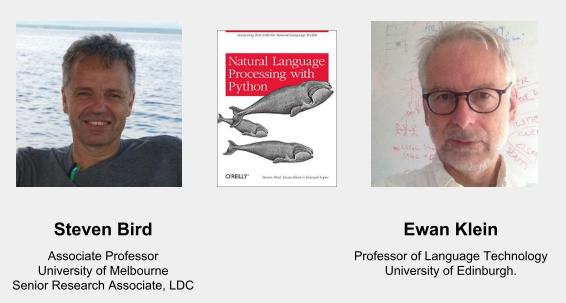
\includegraphics[width=\linewidth,keepaspectratio]{bird}
\end{center}
\end{frame}

%%%%%%%%%%%%%%%%%%%%%%%%%%%%%%%%%%%%%%%%%%%%%%%%%%%%%%%%%%%%%%%%%%%%%%%%%%%%%%%%%%
\begin{frame}[fragile]\frametitle{Batteries Included}
\begin{center}

\includegraphics[width=\linewidth,keepaspectratio]{battery}
\end{center}
NLTK = Corpora + Algorithms\\
Ready for Research!
\end{frame}

%%%%%%%%%%%%%%%%%%%%%%%%%%%%%%%%%%%%%%%%%%%%%%%%%%%%%%%%%%%%%%%%%%%%%%%%%%%%%%%%%%%
%\begin{frame}[fragile]\frametitle{Natural Language Toolkit}
%  \begin{itemize}
%    \item facilitate access to data
%%      \note[item]{only write a format reader once, then share}
%%      \note[item]{reading a format correctly is harder than you think, cf csv}
%    \item standard algorithms
%%      \note[item]{getting into NLP requires knowledge of linguistics, CS, AI which is hard to get}
%%      \note[item]{clarity of Python: people can read the reference implementation, try it, reimplement it...}
%    \item tutorials
%%      \note[item]{major textbooks are formidable, encyclopedic}
%%      \note[item]{we've selected useful core, and provided practical learning materials (book, demos, source)}
%%      \note[item]{practical: learning-by-doing; theoretically sound: stepping stone to research literature}
%    \item contents
%%      \note[item]{50k lines of code, 300Mb datasets, 380pp book}
%    \item evolution: beginnings, redesign
%%      \note[item]{teaching NLP, got too heavy using nested dictionaries, people ended up ''programming in NLTK'', rather than programming in Python using NLTK where needed}
%%      \note[item]{NLTK-Lite: completely reimplemented, simpler structure, uses new language features like set, generator expressions, defaultdict, elementtree}
%%      \note[item]{Design philosophy: interface definitions, lightweight reference implementations, utilities for common tasks}
%  \end{itemize}
%\end{frame}

%%%%%%%%%%%%%%%%%%%%%%%%%%%%%%%%%%%%%%%%%%%%%%%%%%%%%%%%%%%%%%%%%%%%%%%%%%%%%%%%%%
\begin{frame}[fragile]\frametitle{NLTK: What you get \ldots}
  \begin{itemize}
    \item Distributions:
      \textit{Windows, Mac OSX, Unix, data, documentation}
         \item  Suite of libraries for a variety of academic text processing tasks:
           \begin{itemize}
    \item tokenization, stemming, tagging,
    \item  chunking, parsing, classification,
    \item  language modeling, logical semantics
      \end{itemize}
    \item Pedagogical resources for teaching NLP theory in 
Python \ldots
  \end{itemize}
\end{frame}




%%%%%%%%%%%%%%%%%%%%%%%%%%%%%%%%%%%%%%%%%%%%%%%%%%%%%%%%%%%%%%%%%%%%%%%%%%%%%%%%%%
\begin{frame}[fragile]\frametitle{What is NLTK not?}
  \begin{itemize}
    \item Production ready out of the box
    \item Lightweight
    \item Generally applicable
    \item Magic
  \end{itemize}
\end{frame}

%%%%%%%%%%%%%%%%%%%%%%%%%%%%%%%%%%%%%%%%%%%%%%%%%%%%%%%%%%%%%%%%%%%%%%%%%%%%%%%%%%
\begin{frame}[fragile]\frametitle{The Good}
  \begin{itemize}
    \item Preprocessing: segmentation, tokenization, PoS tagging
    \item  Word level processing: WordNet, Lemmatization, Stemming, NGram, Chunking, Named Entity Recognition
    \item  Utilities: Tree, FreqDist, ConditionalFreqDist
    \item Classification: Maximum Entropy, Naive Bayes, Decision Tree
  \end{itemize}
\end{frame}

%%%%%%%%%%%%%%%%%%%%%%%%%%%%%%%%%%%%%%%%%%%%%%%%%%%%%%%%%%%%%%%%%%%%%%%%%%%%%%%%%%
\begin{frame}[fragile]\frametitle{The Bad}
  \begin{itemize}
    \item Syntactic Parsing: No included grammar (not a black box)
    \item  Feature/Dependency Parsing: No included feature grammar
    \item The sem package: Toy only 
    \item Lots of extra stuff: papers, chat programs, alignments, etc
  \end{itemize}
\end{frame}



%%%%%%%%%%%%%%%%%%%%%%%%%%%%%%%%%%%%%%%%%%%%%%%%%%%%%%%%%%%%%%%%%%%%%%%%%%%%%%%%%%
\begin{frame}[fragile]\frametitle{NLTK: Who it is for...}
  \begin{itemize}
    \item People who want to learn how to:
    \begin{itemize}
      \item write programs
      \item to analyze written language
    \end{itemize}
    \item Does not presume programming abilities:
    \begin{itemize}
      \item working examples
      \item graded exercises
    \end{itemize}
    \item Experienced programmers:
    \begin{itemize}
      \item quickly learn Python (if necessary)
      \item Python features for NLP
      \item NLP algorithms and data structures
    \end{itemize}
  \end{itemize}
\end{frame}

%%%%%%%%%%%%%%%%%%%%%%%%%%%%%%%%%%%%%%%%%%%%%%%%%%%%%%%%%%%%%%%%%%%%%%%%%%%%%%%%%%%
%\begin{frame}[fragile]\frametitle{NLTK: What you will learn...}
%  \begin{itemize}
%    \item How to analyze language data
%    \item Key concepts from linguistic description and analysis
%    \item How linguistic knowledge is used in NLP components
%    \item Data structures and algorithms used in NLP and linguistic data management
%    \item Standard corpora and their use in formal evaluation
%    \item Organization of the field of NLP
%    \item Skills in Python programming for NLP
%  \end{itemize}
%\end{frame}

%%%%%%%%%%%%%%%%%%%%%%%%%%%%%%%%%%%%%%%%%%%%%%%%%%%%%%%%%%%%%%%%%%%%%%%%%%%%%%%%%%%
%\begin{frame}[fragile]\frametitle{NLTK: Your likely goals...}
%\small
%\begin{tabular}{p{0.18\linewidth}|p{0.38\linewidth}|p{0.38\linewidth}}
%\textbf{Goals} & \multicolumn{2}{c}{\textbf{Background}} \\
%& \textit{Arts and Humanities} & \textit{Science and Engineering} \\ \hline
%\textbf{Language Analysis}
%& Programming to manage language data, explore linguistic models, and test empirical claims
%& Language as a source of interesting problems in data modeling, data mining, and knowledge discovery\\ \hline
%\textbf{Language Technology}
%& Learning to program, with applications to familiar problems, to work in language technology or other technical field
%& Knowledge of linguistic algorithms and data structures for high quality, maintainable language processing software\\
%\end{tabular}
%\end{frame}

%%%%%%%%%%%%%%%%%%%%%%%%%%%%%%%%%%%%%%%%%%%%%%%%%%%%%%%%%%%%%%%%%%%%%%%%%%%%%%%%%%%
%\begin{frame}[fragile]
%  \begin{center}
%    {\Large NTLTK Book}
%  \end{center}
%\end{frame}

%%%%%%%%%%%%%%%%%%%%%%%%%%%%%%%%%%%%%%%%%%%%%%%%%%%%%%%%%%%%%%%%%%%%%%%%%%%%%%%%%%%
%\begin{frame}[fragile]\frametitle{Nltk Book Philosophy}
%  \begin{itemize}
%    \item Practical
%    \item Programming
%    \item Principled
%    \item Pragmatic
%    \item Pleasurable
%    \item Portal    
%  \end{itemize}
%\end{frame}
%
%%%%%%%%%%%%%%%%%%%%%%%%%%%%%%%%%%%%%%%%%%%%%%%%%%%%%%%%%%%%%%%%%%%%%%%%%%%%%%%%%%%
%\begin{frame}[fragile]\frametitle{Nltk Book Structure}
%  \begin{itemize}
%    \item Three parts:
%    \begin{itemize}
%      \item \textbf{Basics:} text processing, tokenization, tagging,
%        lexicons, language engineering, text classification
%      \item \textbf{Parsing:} phrase structure, trees, grammars, chunking, parsing
%      \item \textbf{Advanced Topics:} selected topics in greater depth:
%        feature-based grammar, unification, semantics, linguistic data management
%    \end{itemize}
%    \item each part: chapter on programming; three chapters on NLP
%    \item each chapter: motivation, sections, graded exercises, summary, further reading
%  \end{itemize}
%\end{frame}
%
%%%%%%%%%%%%%%%%%%%%%%%%%%%%%%%%%%%%%%%%%%%%%%%%%%%%%%%%%%%%%%%%%%%%%%%%%%%%%%%%%%%
%\begin{frame}[fragile]\frametitle{Choice of Python for NLP/NLTK}
%  \begin{itemize}
%    \item Simple yet powerful, shallow learning curve
%    \item Object-oriented: encapsulation, re-use
%    \item Scripting language, facilitates interactive exploration
%    \item Excellent functionality for processing linguistic data
%    \item Extensive standard library, incl graphics, web, numerical processing
%  \end{itemize}
%\end{frame}
%
%%%%%%%%%%%%%%%%%%%%%%%%%%%%%%%%%%%%%%%%%%%%%%%%%%%%%%%%%%%%%%%%%%%%%%%%%%%%%%%%%%%
%\begin{frame}[fragile]\frametitle{Python Example}
%
%\begin{lstlisting}
% import sys
% for line in sys.stdin.readlines():
%     for word in line.split():
%         if word.endswith('ing'):
%             print word
%\end{lstlisting}
%
%\begin{itemize}
%\item whitespace: nesting lines of code; scope
%\item object-oriented: attributes, methods (e.g. \texttt{line})
%\item readable
%\end{itemize}
%\end{frame}
%
%%%%%%%%%%%%%%%%%%%%%%%%%%%%%%%%%%%%%%%%%%%%%%%%%%%%%%%%%%%%%%%%%%%%%%%%%%%%%%%%%%%
%\begin{frame}[fragile]\frametitle{Comparison with Perl}
%
%\begin{lstlisting}
%  while (<>) {
%      foreach my $word (split) {
%          if ($word =~ /ing$/) {
%              print ''$word\n'';
%          }
%      }
%  }
%\end{lstlisting}
%
%\begin{itemize}
%\item syntax is obscure: \textit{what are:} \verb|<> $ my split| ?
%\item ``it is quite easy in Perl to write programs that simply
%  look like raving gibberish, even to experienced Perl programmers''
%  (Hammond \textit{Perl Programming for Linguists} 2003:47)
%\item large programs difficult to maintain, reuse
%\end{itemize}
%\end{frame}
%
%%%%%%%%%%%%%%%%%%%%%%%%%%%%%%%%%%%%%%%%%%%%%%%%%%%%%%%%%%%%%%%%%%%%%%%%%%%%%%%%%%%
%\begin{frame}[fragile]\frametitle{What NLTK adds to Python}
%
%NLTK defines a basic infrastructure that can be used to build NLP
%programs in Python.  It provides:
%
%\begin{itemize}
%\item Basic classes for representing data relevant to natural language
%  processing
%\item Standard interfaces for performing tasks, such
%  as tokenization, tagging, and parsing
%\item Standard implementations for each task, which
%  can be combined to solve complex problems
%\item Demonstrations (parsers, chunkers, chatbots)
%\item Extensive documentation, including tutorials
%  and reference documentation
%\end{itemize}
%\end{frame}
%
%

%
%%%%%%%%%%%%%%%%%%%%%%%%%%%%%%%%%%%%%%%%%%%%%%%%%%%%%%%%%%%%%%%%%%%%%%%%%%%%%%%%%%%
%\begin{frame}[fragile]\frametitle{NLTK Design: Requirements}
%  \begin{itemize}
%    \item \textbf{Simplicity:} intuitive framework with substantial building blocks
%    \item \textbf{Consistency:} uniform data structures, interfaces --- predictability
%    \item \textbf{Extensibility:} accommodates new components
%      (replicate vs extend exiting functionality)
%    \item \textbf{Modularity:} interaction between components
%    \item \textbf{Well-documented:} substantial documentation
%  \end{itemize}
%\end{frame}
%
%%%%%%%%%%%%%%%%%%%%%%%%%%%%%%%%%%%%%%%%%%%%%%%%%%%%%%%%%%%%%%%%%%%%%%%%%%%%%%%%%%%
%\begin{frame}[fragile]\frametitle{NLTK Design: Non-requirements}
%  \begin{itemize}
%    \item \textbf{Encyclopedic:} has many gaps; opportunity for students to extend it
%    \item \textbf{Efficiency:} not highly optimised for runtime performance
%    \item \textbf{Programming tricks:} avoid in preference for clear implementations
%      (replicate vs extend exiting functionality)
%  \end{itemize}
%\end{frame}

%%%%%%%%%%%%%%%%%%%%%%%%%%%%%%%%%%%%%%%%%%%%%%%%%%%%%%%%%%%%%%%%%%%%%%%%%%%%%%%%%%
\begin{frame}[fragile]\frametitle{Corpora Distributed with NLTK}
  \tiny
  \begin{itemize}
    \item Australian ABC News, 2 genres, 660k words, sentence-segmented
    \item Brown Corpus, 15 genres, 1.15M words, tagged
    \item CMU Pronouncing Dictionary, 127k entries
    \item CoNLL 2000 Chunking Data, 270k words, tagged and chunked
    \item CoNLL 2002 Named Entity, 700k words, pos- and named-entity-tagged (Dutch, Spanish)
    \item Floresta Treebank, 9k sentences (Portuguese)
    \item Genesis Corpus, 6 texts, 200k words, 6 languages
    \item Gutenberg (sel), 14 texts, 1.7M words
    \item Indian POS-Tagged Corpus, 60k words pos-tagged (Bangla, Hindi, Marathi, Telugu)
    \item NIST 1999 Info Extr (sel), 63k words, newswire and named-entity SGML markup
    \item Names Corpus, 8k male and female names
    \item PP Attachment Corpus, 28k prepositional phrases, tagged as noun or verb modifiers
    \item Presidential Addresses, 485k words, formatted text
    \item Roget's Thesaurus, 200k words, formatted text
    \item SEMCOR, 880k words, part-of-speech and sense tagged
    \item SENSEVAL 2, 600k words, part-of-speech and sense tagged
    \item Shakespeare XML Corpus (sel), 8 books
    \item Stopwords Corpus, 2,400 stopwords for 11 languages
    \item Switchboard Corpus (sel), 36 phonecalls, transcribed, parsed
    \item Univ Decl Human Rights, 480k words, 300+ languages
    \item US Pres Addr Corpus, 480k words
    \item Penn Treebank (sel), 40k words, tagged and parsed
    \item TIMIT Corpus (sel), audio files and transcripts for 16 speakers
    \item Wordlist Corpus, 960k words and 20k affixes for 8 languages
    \item WordNet, 145k synonym sets
  \end{itemize}
\end{frame}

% % %%%%%%%%%%%%%%%%%%%%%%%%%%%%%%%%%%%%%%%%%%%%%%%%%%%%%%%%%%%%%%%%%%%%%%%%%%%%%%%%%%%
% % %\begin{frame}[fragile]\frametitle{Python Overview: Defining Lists}
% % %  \small
% % %\begin{itemize}
% % %\item list: ordered sequence of items
% % %\item item: string, number, complex object (e.g. a list)
% % %\item list representation: comma separated items: \verb|['John', 14, 'Sep', 1984]|
% % %\item list initialization:
% % %\begin{lstlisting}
% % %    >>> a = [`colourless', `green', `ideas']
% % %\end{lstlisting}
% % %\item sets the value of variable \texttt{a}
% % %\item to see the its value, do: \texttt{print a}
% % %\item in interactive mode, just type the variable name:
% % %\begin{lstlisting}
% % %  >>> a
% % %  [`colourless', `green',`'ideas']
% % %\end{lstlisting}
% % %\end{itemize}
% % %\end{frame}
% % %
% % %%%%%%%%%%%%%%%%%%%%%%%%%%%%%%%%%%%%%%%%%%%%%%%%%%%%%%%%%%%%%%%%%%%%%%%%%%%%%%%%%%%
% % %\begin{frame}\frametitle{Simple List Operations}
% % %  \small
% % %\begin{itemize}
% % %\item length: \texttt{len()}
% % %\item indexing: \texttt{a[0]}, \texttt{a[1]}
% % %\item indexing from right: \texttt{a[-1]}
% % %\item slices: \texttt{a[1:3]}, \texttt{a[-2:]}
% % %\item concatenation: \texttt{b = a + ['sleep', 'furiously']}
% % %\item sorting: \texttt{b.sort()}
% % %\item reversing: \texttt{b.reverse()}
% % %\item iteration: \texttt{for item in a:}
% % %\item all the above applies to strings as well
% % %\item double indexing: \texttt{b[2][1]}
% % %\item finding index: \texttt{b.index('green')}
% % %\end{itemize}
% % %\end{frame}
% % %
% % %%%%%%%%%%%%%%%%%%%%%%%%%%%%%%%%%%%%%%%%%%%%%%%%%%%%%%%%%%%%%%%%%%%%%%%%%%%%%%%%%%%
% % %\begin{frame}\frametitle{Simple String Operations}
% % %  \small
% % %\begin{itemize}
% % %\item joining: \texttt{c = ' '.join(b)}
% % %\item splitting: \texttt{c.split('r')}
% % %\item lambda expressions: \texttt{lambda x: len(x)}
% % %\item maps: \texttt{map(lambda x: len(x), b)}
% % %\item list comprehensions: \texttt{[(x, len(x)) for x in b]}
% % %\item getting help: \texttt{help(list)}, \texttt{help(str)}
% % %\end{itemize}
% % %\end{frame}
% % %
% % %%%%%%%%%%%%%%%%%%%%%%%%%%%%%%%%%%%%%%%%%%%%%%%%%%%%%%%%%%%%%%%%%%%%%%%%%%%%%%%%%%%
% % %\begin{frame}[fragile]\frametitle{Dictionaries}
% % %  \small
% % %
% % %\begin{itemize}
% % %\item accessing items by their names, e.g. dictionary
% % %\item defining entries:
% % %
% % %\begin{lstlisting}
% % %  >>> d = {}
% % %  >>> d['colourless'] = 'adj'
% % %  >>> d['furiously'] = 'adv'
% % %  >>> d['ideas'] = 'n'
% % %\end{lstlisting}
% % %
% % %\item accessing:
% % %
% % %\begin{lstlisting}
% % %  >>> d.keys()
% % %  ['furiously', 'colourless', 'ideas']
% % %  >>> d['ideas']
% % %  'n'
% % %  >>> d
% % %  {'furiously': 'adv', 'colourless': 'adj', 'ideas': 'n'}
% % %\end{lstlisting}
% % %\end{itemize}
% % %\end{frame}
% % %
% % %%%%%%%%%%%%%%%%%%%%%%%%%%%%%%%%%%%%%%%%%%%%%%%%%%%%%%%%%%%%%%%%%%%%%%%%%%%%%%%%%%%
% % %\begin{frame}[fragile]\frametitle{Dictionaries: Iteration}
% % %
% % %\begin{lstlisting}
% % %  >>> for w in d:
% % %  ...    print ''%s [%s],'' % (w, d[w]),
% % %  furiously [adv], colourless [adj], ideas [n],
% % %\end{lstlisting}
% % %
% % %\begin{itemize}
% % %\item rule of thumb: dictionary entries are like variable names
% % %\item \textit{create} them by assigning to them\\
% % %  \verb|x = 2| (variable), \verb|d['x'] = 2| (dictionary entry)
% % %\item \textit{access} them by reference\\
% % %  \verb|print x| (variable), \verb|print d['x']| (dictionary entry)
% % %\end{itemize}
% % %\end{frame}
% % %
% % %%%%%%%%%%%%%%%%%%%%%%%%%%%%%%%%%%%%%%%%%%%%%%%%%%%%%%%%%%%%%%%%%%%%%%%%%%%%%%%%%%%
% % %\begin{frame}[fragile]\frametitle{Dictionaries: Example: Counting Word Occurrences}
% % %\scriptsize
% % %
% % %\begin{lstlisting}
% % %  >>> import nltk
% % %  >>> count = {}
% % %  >>> for word in nltk.corpus.gutenberg.words('shakespeare-macbeth'):
% % %  ...     word = word.lower()
% % %  ...     if word not in count:
% % %  ...         count[word] = 0
% % %  ...     count[word] += 1
% % %\end{lstlisting}
% % %
% % %Now inspect the dictionary:
% % %
% % %\begin{lstlisting}
% % %  >>> print count['scotland']
% % %  12
% % %  >>> frequencies = [(freq, word) for (word, freq) in count.items()]
% % %  >>> frequencies.sort()
% % %  >>> frequencies.reverse()
% % %  >>> print frequencies[:20]
% % %  [(1986, ','), (1245, '.'), (692, 'the'), (654, '''''), (567, 'and'), (482, ':'), (399, 'to'), (365, 'of'), (360, 'i'), (255, 'a'), (246, 'that'), (242, '?'), (224, 'd'), (218, 'you'), (213, 'in'), (207, 'my'), (198, 'is'), (170, 'not'), (165, 'it'), (156, 'with')]
% % %\end{lstlisting}
% % %\end{frame}
% % %%
% % %%%%%%%%%%%%%%%%%%%%%%%%%%%%%%%%%%%%%%%%%%%%%%%%%%%%%%%%%%%%%%%%%%%%%%%%%%%%%%%%%%%
% % %\begin{frame}[fragile]\frametitle{Defining Functions}
% % %\scriptsize
% % %\begin{itemize}
% % %\item part of a program needs to be used several times over
% % %\item e.g. form plural of singular noun, to be done in several places
% % %  in a program
% % %\item localize this work inside a \textit{function}
% % %\item also helps readability, reusability
% % %
% % %\begin{lstlisting}
% % %  >>> def plural(word):
% % %  ...     if word[-1] == 'y':
% % %  ...         return word[:-1] + 'ies'
% % %  ...     elif word[-1] in 'sx':
% % %  ...         return word + 'es'
% % %  ...     elif word[-2:] in ['sh', 'ch']:
% % %  ...         return word + 'es'
% % %  ...     elif word[-2:] == 'an':
% % %  ...         return word[:-2] + 'en'
% % %  ...     return word + 's'
% % %  >>> plural('fairy')
% % %  'fairies'
% % %  >>> plural('woman')
% % %  'women'
% % %\end{lstlisting}
% % %\end{itemize}
% % %\end{frame}
% % %
% % %%%%%%%%%%%%%%%%%%%%%%%%%%%%%%%%%%%%%%%%%%%%%%%%%%%%%%%%%%%%%%%%%%%%%%%%%%%%%%%%%%%
% % %\begin{frame}[fragile]\frametitle{Defining Modules}
% % %
% % %\begin{lstlisting}
% % %def parsed(files):
% % %    for file in files:
% % %        path = os.path.join(get_basedir(), ''treebank'', file)
% % %        s = open(path).read()
% % %        for t in tokenize.blankline(s):
% % %            yield tree.bracket_parse(t)
% % %\end{lstlisting}
% % %\end{frame}
% % %
% % %%%%%%%%%%%%%%%%%%%%%%%%%%%%%%%%%%%%%%%%%%%%%%%%%%%%%%%%%%%%%%%%%%%%%%%%%%%%%%%%%%%
% % %\begin{frame}[fragile]\frametitle{Algorithm Design}
% % %  \small
% % %
% % %  \begin{itemize}
% % %  \item \textit{algorithm}: a ''recipe'' for solving a problem
% % %  \item e.g. to multiply 16 by 12 we might use any of the following methods:
% % %
% % %    \begin{itemize}
% % %    \item Add 16 to itself 12 times over
% % %    \item Perform ''long multiplication'', starting with the least-significant
% % %      digits of both numbers
% % %    \item Look up a multiplication table
% % %    \item Repeatedly halve the first number and double the second,
% % %      16*12 = 8*24 = 4*48 = 2*96 = 192
% % %    \item Do 10*12 to get 120, then add 6*12
% % %    \end{itemize}
% % %
% % %  \item computation time, intermediate storage
% % %  \item brute-force, divide-and-conquer, dynamic programming, greedy search
% % %  \item Textbook: Levitin, Anany (2003) \textit{Introduction to the Design and
% % %      Analysis of Algorithms}
% % %  \end{itemize}
% % %\end{frame}
% % %
% % %%%%%%%%%%%%%%%%%%%%%%%%%%%%%%%%%%%%%%%%%%%%%%%%%%%%%%%%%%%%%%%%%%%%%%%%%%%%%%%%%%%
% % %\begin{frame}[fragile]\frametitle{Sorting Algorithms}
% % %
% % %\begin{itemize}
% % %\item Many algorithms for sorting
% % %\item Illustrates the difference in algorithm complexity
% % %
% % %\begin{lstlisting}
% % %  >>> from random import shuffle
% % %  >>> from nltk.misc import sort
% % %  >>> a = range(1000)
% % %  >>> shuffle(a); sort.bubble(a)
% % %  250918
% % %  >>> shuffle(a); sort.merge(a)
% % %  6175
% % %  >>> shuffle(a); sort.quick(a)
% % %  2378
% % %\end{lstlisting}
% % %\end{itemize}
% % %\end{frame}
%

%%%%%%%%%%%%%%%%%%%%%%%%%%%%%%%%%%%%%%%%%%%%%%%%%%%%%%%%%%%%%%%%%%%%%%%%%%%%%%%%%%
\begin{frame}[fragile]\frametitle{Getting started}
Installation:
  \begin{lstlisting}
conda install -c conda-forge nltk or pip install nltk
>>> import nltk
>>> nltk.download()
  \end{lstlisting}
  
Choose ``Popular'' collection
\begin{center}
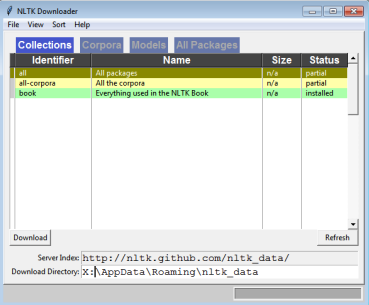
\includegraphics[width=0.4\linewidth,keepaspectratio]{nltkdownload}
\end{center}

For the most recent instructions always look at http://www.nltk.org/install.html
\end{frame}

%%%%%%%%%%%%%%%%%%%%%%%%%%%%%%%%%%%%%%%%%%%%%%%%%%%%%%%%%%%%%%%%%%%%%%%%%%%%%%%%%%
\begin{frame}[fragile]\frametitle{Books}
\begin{center}
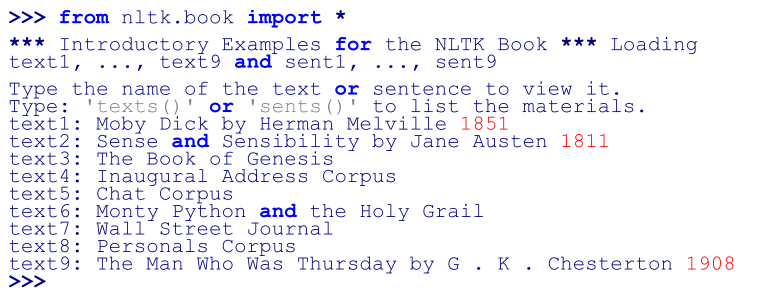
\includegraphics[width=0.8\linewidth,keepaspectratio]{nltkbooks}
\end{center}

Note: At times, it may ask you to download few resources, do so.
\end{frame}

%%%%%%%%%%%%%%%%%%%%%%%%%%%%%%%%%%%%%%%%%%%%%%%%%%%%%%%%%%%%%%%%%%%%%%%%%%%%%%%%%%
\begin{frame}[fragile]\frametitle{Texts}
\begin{center}
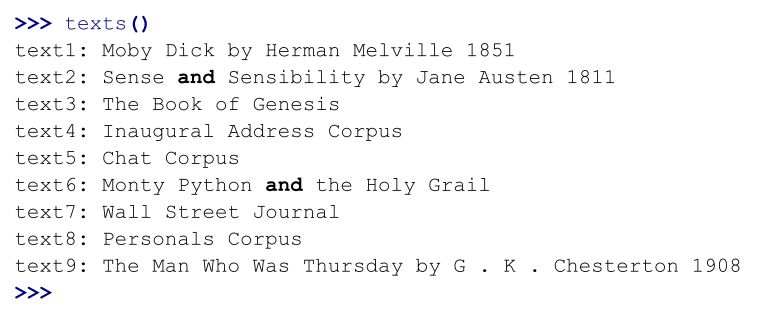
\includegraphics[width=0.8\linewidth,keepaspectratio]{nltktexts}
\end{center}
\end{frame}

%%%%%%%%%%%%%%%%%%%%%%%%%%%%%%%%%%%%%%%%%%%%%%%%%%%%%%%%%%%%%%%%%%%%%%%%%%%%%%%%%%%
%\begin{frame}[fragile]\frametitle{Sentences}
%\begin{center}
%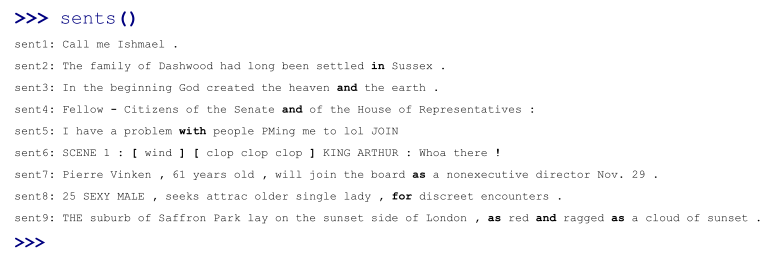
\includegraphics[width=0.8\linewidth,keepaspectratio]{nltksents}
%\end{center}
%\end{frame}

%%%%%%%%%%%%%%%%%%%%%%%%%%%%%%%%%%%%%%%%%%%%%%%%%%%%%%%%%%%%%%%%%%%%%%%%%%%%%%%%%%
%\begin{frame}[fragile]\frametitle{Sentences}
%\begin{center}
%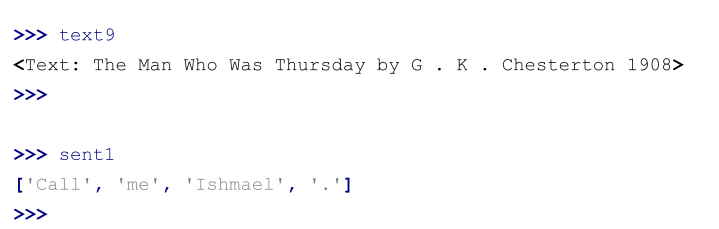
\includegraphics[width=0.8\linewidth,keepaspectratio]{nltksent1}
%\end{center}
%\end{frame}


%%%%%%%%%%%%%%%%%%%%%%%%%%%%%%%%%%%%%%%%%%%%%%%%%%%%%%%%%%%%%%%%%%%%%%%%%%%%%%%%%%
\begin{frame}[fragile]\frametitle{Try out}
Counting words:
      \begin{lstlisting}
len(set(text1))
  \end{lstlisting}
  
``text1", for for that matter, the corpora variables like text1, are actually class objects. Simple use of them, returns list of tokens (iterator). This is similar to the way python dict object is used in a for look. Simple dict object returns `keys'.

\end{frame}


%%%%%%%%%%%%%%%%%%%%%%%%%%%%%%%%%%%%%%%%%%%%%%%%%%%%%%%%%%%%%%%%%%%%%%%%%%%%%%%%%%
\begin{frame}[fragile]\frametitle{Concordance}
API:
\begin{lstlisting}
text.similar(str)
concordance(str) # shows words around as well
len(text)
len(set(text))
text.collocations()
\end{lstlisting}
  
\begin{center}
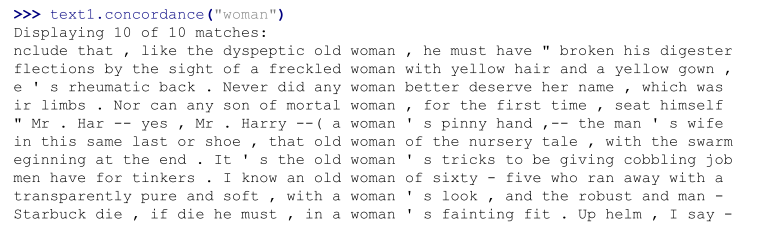
\includegraphics[width=0.8\linewidth,keepaspectratio]{nltkconcord}
\end{center}
\end{frame}

%%%%%%%%%%%%%%%%%%%%%%%%%%%%%%%%%%%%%%%%%%%%%%%%%%%%%%%%%%%%%%%%%%%%%%%%%%%%%%%%%%%
%\begin{frame}[fragile]\frametitle{Concordance}
%\begin{center}
%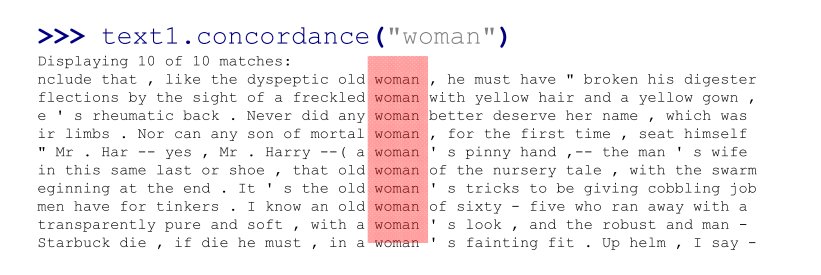
\includegraphics[width=\linewidth,keepaspectratio]{nltkconcord1}
%\end{center}
%\end{frame}

%%%%%%%%%%%%%%%%%%%%%%%%%%%%%%%%%%%%%%%%%%%%%%%%%%%%%%%%%%%%%%%%%%%%%%%%%%%%%%%%%%
\begin{frame}[fragile]\frametitle{Lexical Diversity}

Write own function \ldots

\begin{center}
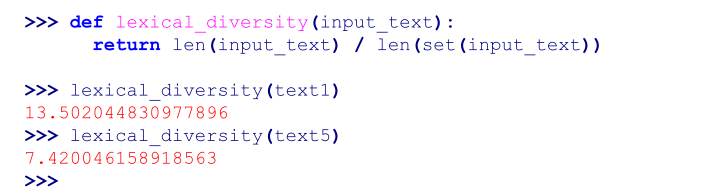
\includegraphics[width=0.8\linewidth,keepaspectratio]{lexdiv}
\end{center}
\end{frame}



% %%%%%%%%%%%%%%%%%%%%%%%%%%%%%%%%%%%%%%%%%%%%%%%%%%%%%%%%%%%%%%%%%%%%%%%%%%%%%%%%%%
% \begin{frame}[fragile]\frametitle{Exercise}
% Write a program that :
% \begin{itemize}
% \item Reads a large text file (corpus), splits into words/tokens
% \item Make a dictionary of words and their frequencies
% \item Write the dictionary to another text file.
% \item Alter the dictionary so that it contains only words which are longer than 5 characters and start with `b'
% \end{itemize}
% \end{frame}


%%%%%%%%%%%%%%%%%%%%%%%%%%%%%%%%%%%%%%%%%%%%%%%%%%%%%%%%%%%%%%%%%%%%%%%%%%%%%%%%%%
\begin{frame}[fragile]\frametitle{Try out}
  Finding frequency of words:

  \begin{lstlisting}
fd = FreqDist(text)
fd
\end{lstlisting}

Gives words and their frequencies.

Find 20 Most Frequent Words in a Text

  \begin{lstlisting}
fd.most_common(20)
\end{lstlisting}


% {\scriptsize\begin{lstlisting}
% >>> counts = defaultdict(int)
% >>> for word in text.split():
% ...     counts[word] += 1
% >>> ranked_words = sorted(counts.items, key=itemgetter(1))
% >>> print [word for (word,count) in reversed(ranked_words)][:20]
% \end{lstlisting}}

% Note: defaultdict; sorting tuples, list comprehensions

% {\scriptsize\begin{lstlisting}
% >>> print FreqDist(tokenize.wordpunct(text)).sorted()[:20]
% \end{lstlisting}}
\end{frame}



%%%%%%%%%%%%%%%%%%%%%%%%%%%%%%%%%%%%%%%%%%%%%%%%%%%%%%%%%%%%%%%%%%%%%%%%%%%%%%%%%%
\begin{frame}[fragile]\frametitle{Collocations}
\begin{itemize}
\item Collocations: a sequence of words that occur together more than often.
\item Thus, not all the bi/tri-grams are collocations
\end{itemize}
{\small
\begin{lstlisting}
>>> text1.collocations(5)

Sperm Whale; Moby Dick; White Whale: old man; Captain Ahab
\end{lstlisting}}
\end{frame}

%%%%%%%%%%%%%%%%%%%%%%%%%%%%%%%%%%%%%%%%%%%%%%%%%%%%%%%%%%%%%%%%%%%%%%%%%%%%%%%%%%
\begin{frame}[fragile]\frametitle{N-grams}
\begin{itemize}
\item Bi-grams: a sequence of 2 words
\item Tri-grams : a sequence of 3 words
\item N-grams: a sequence of n words
\end{itemize}
{\small
\begin{lstlisting}
for pair in nltk.bigrams([`more', `is',`said','than','done']):
	print(pair)
	
(`more', `is')
(`is','said')
(`said','than')
(`than','done')
\end{lstlisting}}
\end{frame}


%%%%%%%%%%%%%%%%%%%%%%%%%%%%%%%%%%%%%%%%%%%%%%%%%%%%%%%%%%%%%%%%%%%%%%%%%%%%%%%%%%%%%
%%%\begin{frame}[fragile]\frametitle{Example: TIMIT}
%%%\begin{itemize}
%%%\item TI (Texas Instruments) + MIT
%%%\item balance
%%%\item sentence selection
%%%\item layers of annotation
%%%\item speaker demographics, lexicon
%%%\item combination of time-series and record-structured data
%%%\item programs for speech corpus
%%%\end{itemize}
%%%\end{frame}
%%%
%%%
%%%%%%%%%%%%%%%%%%%%%%%%%%%%%%%%%%%%%%%%%%%%%%%%%%%%%%%%%%%%%%%%%%%%%%%%%%%%%%%%%%%%%
%%%\begin{frame}[fragile]
%%%\frametitle{Example: TIMIT}
%%%\scriptsize
%%%\begin{lstlisting}
%%%    >>> phonetic = nltk.corpus.timit.phones(dr1-fvmh0/sa1')
%%%    >>> phonetic
%%%    ['h#', 'sh', 'iy', 'hv', 'ae', 'dcl', 'y', 'ix', 'dcl', 'd', 'aa', 'kcl',
%%%    's', 'ux', 'tcl', 'en', 'gcl', 'g', 'r', 'iy', 's', 'iy', 'w', 'aa',
%%%    'sh', 'epi', 'w', 'aa', 'dx', 'ax', 'q', 'ao', 'l', 'y', 'ih', 'ax', 'h#']
%%%    >>> nltk.corpus.timit.word_times('dr1-fvmh0/sa1')
%%%    [('she', 7812, 10610), ('had', 10610, 14496), ('your', 14496, 15791),
%%%    ('dark', 15791, 20720), ('suit', 20720, 25647), ('in', 25647, 26906),
%%%    ('greasy', 26906, 32668), ('wash', 32668, 37890), ('water', 38531, 42417),
%%%    ('all', 43091, 46052), ('year', 46052, 50522)]
%%%\end{lstlisting}
%%%\end{frame}
%%%
%%%%%%%%%%%%%%%%%%%%%%%%%%%%%%%%%%%%%%%%%%%%%%%%%%%%%%%%%%%%%%%%%%%%%%%%%%%%%%%%%%%%%
%%%\begin{frame}[fragile]
%%%\frametitle{Example: TIMIT}
%%%\scriptsize
%%%\begin{lstlisting}
%%%    >>> timitdict = nltk.corpus.timit.transcription_dict()
%%%    >>> timitdict['greasy'] + timitdict['wash'] + timitdict['water']
%%%    ['g', 'r', 'iy1', 's', 'iy', 'w', 'ao1', 'sh', 'w', 'ao1', 't', 'axr']
%%%    >>> phonetic[17:30]
%%%    ['g', 'r', 'iy', 's', 'iy', 'w', 'aa', 'sh', 'epi', 'w', 'aa', 'dx', 'ax']
%%%
%%%    >>> nltk.corpus.timit.spkrinfo('dr1-fvmh0')
%%%    SpeakerInfo(id='VMH0', sex='F', dr='1', use='TRN', recdate='03/11/86',
%%%    birthdate='01/08/60', ht='5\'05"', race='WHT', edu='BS',
%%%    comments='BEST NEW ENGLAND ACCENT SO FAR')
%%%\end{lstlisting}
%%%\end{frame}
%%
%%%%%%%%%%%%%%%%%%%%%%%%%%%%%%%%%%%%%%%%%%%%%%%%%%%%%%%%%%%%%%%%%%%%%%%%%%%%%%%%%%%%
%%\begin{frame}[fragile]\frametitle{Data Cleansing: Accessing Spreadsheets}
%%\scriptsize
%%\begin{lstlisting}
%%dict.csv:
%%"sleep","sli:p","v.i","a condition of body and mind ..."
%%"walk","wo:k","v.intr","progress by lifting and setting down each foot ..."
%%"wake","weik","intrans","cease to sleep"
%%
%%    >>> import csv
%%    >>> file = open("dict.csv", "rb")
%%    >>> for row in csv.reader(file):
%%    ...     print row
%%    ['sleep', 'sli:p', 'v.i', 'a condition of body and mind ...']
%%    ['walk', 'wo:k', 'v.intr', 'progress by lifting and setting down each foot ...']
%%    ['wake', 'weik', 'intrans', 'cease to sleep']
%%\end{lstlisting}
%%\end{frame}
%%
%%%%%%%%%%%%%%%%%%%%%%%%%%%%%%%%%%%%%%%%%%%%%%%%%%%%%%%%%%%%%%%%%%%%%%%%%%%%%%%%%%%%
%%\begin{frame}[fragile]\frametitle{Data Cleansing: Validation}
%%\small
%%\begin{lstlisting}
%%    def undefined_words(csv_file):
%%        import csv
%%        lexemes = set()
%%        defn_words = set()
%%        for row in csv.reader(open(csv_file)):
%%            lexeme, pron, pos, defn = row
%%            lexemes.add(lexeme)
%%            defn_words.union(defn.split())
%%        return sorted(defn_words.difference(lexemes))
%%        
%%    >>> print undefined_words("dict.csv")
%%    ['...', 'a', 'and', 'body', 'by', 'cease',
%%     'condition', 'down', 'each', 'foot',
%%     'lifting', 'mind', 'of', 'progress',
%%     'setting', 'to']
%%\end{lstlisting}
%%\end{frame}
%%
%%%%%%%%%%%%%%%%%%%%%%%%%%%%%%%%%%%%%%%%%%%%%%%%%%%%%%%%%%%%%%%%%%%%%%%%%%%%%%%%%%%%
%%\begin{frame}[fragile]\frametitle{Data Cleansing: Accessing Web Text}
%%
%%\scriptsize
%%\begin{lstlisting}
%%>>> import urllib, nltk
%%>>> html = urllib.urlopen('http://en.wikipedia.org/').read()
%%>>> text = nltk.clean_html(html)
%%>>> text.split()
%%['Wikimedia', 'Error', 'WIKIMEDIA', 'FOUNDATION', 'Fout', 'Fel',
%%'Fallo', '\xe9\x94\x99\xe8\xaf\xaf', '\xe9\x8c\xaf\xe8\xaa\xa4',
%%'Erreur', 'Error', 'Fehler', '\xe3\x82\xa8\xe3\x83\xa9\xe3\x83\xbc',
%%'B\xc5\x82\xc4\x85d', 'Errore', 'Erro', 'Chyba', 'EnglishThe',
%%'Wikimedia', 'Foundation', 'servers', 'are', 'currently',
%%'experiencing', 'technical', 'difficulties.The', 'problem', 'is',
%%'most', 'likely', 'temporary', 'and', 'will', 'hopefully', 'be',
%%'fixed', 'soon.', 'Please', 'check', 'back', 'in', 'a', 'few',
%%'minutes.For', 'further', 'information,', 'you', 'can', 'visit',
%%'the', 'wikipedia', 'channel', 'on', 'the', 'Freenode', 'IRC', ...
%%\end{lstlisting}
%%\end{frame}
%%
%%
%%%%%%%%%%%%%%%%%%%%%%%%%%%%%%%%%%%%%%%%%%%%%%%%%%%%%%%%%%%%%%%%%%%%%%%%%%%%%%%%%%%%
%%\begin{frame}[fragile]\frametitle{Accessing Toolbox Data}
%%
%%\begin{itemize}
%%\item scan the file, convert into tree object
%%\item preserves order of fields, gives array and XPath-style access
%%\end{itemize}
%%
%%\scriptsize
%%\begin{lstlisting}
%%>>> from nltk.corpus import toolbox
%%>>> lexicon = toolbox.xml('rotokas.dic')
%%\end{lstlisting}
%%\end{frame}
%%
%%%%%%%%%%%%%%%%%%%%%%%%%%%%%%%%%%%%%%%%%%%%%%%%%%%%%%%%%%%%%%%%%%%%%%%%%%%%%%%%%%%%
%%\begin{frame}[fragile]\frametitle{Accessing with Indexes}
%%
%%\begin{lstlisting}
%%>>> lexicon[3][0] 
%%<Element lx at 77bd28>
%%>>> lexicon[3][0].tag
%%'lx'
%%>>> lexicon[3][0].text
%%'kaa'
%%\end{lstlisting}
%%\end{frame}
%%
%%%%%%%%%%%%%%%%%%%%%%%%%%%%%%%%%%%%%%%%%%%%%%%%%%%%%%%%%%%%%%%%%%%%%%%%%%%%%%%%%%%%
%%\begin{frame}[fragile]\frametitle{Accessing with Indexes (cont)}
%%
%%\scriptsize
%%\begin{lstlisting}
%%>>> print nltk.corpus.reader.toolbox.to_sfm_string(lexicon[3])
%%\lx kaa
%%\ps N.M
%%\cl isi
%%\ge cooking banana
%%\gp banana bilong kukim
%%\sf FLORA
%%\dt 12/Feb/2005
%%\ex Taeavi iria kaa isi kovopaueva kaparapasia.
%%\xp Taeavi i bin planim gaden banana bilong kukim tasol long paia.
%%\xe Taeavi planted banana in order to cook it.
%%\end{lstlisting}
%%\end{frame}
%%
%%%%%%%%%%%%%%%%%%%%%%%%%%%%%%%%%%%%%%%%%%%%%%%%%%%%%%%%%%%%%%%%%%%%%%%%%%%%%%%%%%%%
%%\begin{frame}[fragile]\frametitle{Accessing with Paths}
%%
%%\scriptsize
%%\begin{lstlisting}
%%>>> [lexeme.text.lower() for lexeme in lexicon.findall('record/lx')]
%%['kaa', 'kaa', 'kaa', 'kaakaaro', 'kaakaaviko', 'kaakaavo', 'kaakaoko',
%%'kaakasi', 'kaakau', 'kaakauko', 'kaakito', 'kaakuupato', ..., 'kuvuto']
%%\end{lstlisting}
%%
%%\small
%%\begin{itemize}
%%\item lexicon is a series of \texttt{record} objects
%%\item each contains field objects, such as \texttt{lx} and \texttt{ps}
%%\item address all the lexemes: \texttt{record/lx}
%%\end{itemize}
%%\end{frame}
%%
%%%%%%%%%%%%%%%%%%%%%%%%%%%%%%%%%%%%%%%%%%%%%%%%%%%%%%%%%%%%%%%%%%%%%%%%%%%%%%%%%%%%
%%\begin{frame}[fragile]\frametitle{Data Cleansing: Toolbox}
%%
%%\begin{itemize}
%%\item Tokenization
%%\item Stemming
%%\item Lemmatization
%%\item Tagging
%%\item Parsing 
%%\item Chunking 
%%\item Adding missing fields 
%%\end{itemize}
%%\end{frame}
%%
%%%%%%%%%%%%%%%%%%%%%%%%%%%%%%%%%%%%%%%%%%%%%%%%%%%%%%%%%%%%%%%%%%%%%%%%%%%%%%%%%%%%
%%\begin{frame}[fragile]\frametitle{Tokenization}
%%
%%\scriptsize
%%\begin{lstlisting}
%%>>> tokens = nltk.word_tokenize(raw)
%%>>> tagalog_tokens = nltk.Text(tokens)
%%>>> tagalog_tokens = set(sample.lower() for sample in tagalog_tokens)
%%\end{lstlisting}
%%
%%\small
%%\begin{itemize}
%%\item 	Breaking up of string into words and punctuations
%%\end{itemize}
%%\end{frame}
%%
%%
%%%%%%%%%%%%%%%%%%%%%%%%%%%%%%%%%%%%%%%%%%%%%%%%%%%%%%%%%%%%%%%%%%%%%%%%%%%%%%%%%%%%
%%\begin{frame}[fragile]\frametitle{Stemming}
%%
%%\scriptsize
%%\begin{lstlisting}
%%>>> def stem(word):
%%...     for suffix in ['ing', 'ly', 'ed', 'ious', 'ies', 'ive', 'es', 's', 'ment']:
%%...             if word.endswith(suffix):
%%...                     return word[:-len(suffix)]
%%...     return word
%%... 
%%>>> stem('reading')
%%'read'
%%>>> stem('moment')
%%'mo'
%%\end{lstlisting}
%%
%%\small
%%\begin{itemize}
%%\item 	Normalize words into its base form, result may not be the 'root' word
%%\end{itemize}
%%\end{frame}
%%
%%%%%%%%%%%%%%%%%%%%%%%%%%%%%%%%%%%%%%%%%%%%%%%%%%%%%%%%%%%%%%%%%%%%%%%%%%%%%%%%%%%%
%%\begin{frame}[fragile]\frametitle{Lemmatization}
%%
%%\scriptsize
%%\begin{lstlisting}
%%>>> def stem(word):
%%...     for suffix in ['ing', 'ly', 'ed', 'ious', 'ies', 'ive', 'es', 's', 'ment']:
%%...             if word.endswith(suffix) and word[:-len(suffix)] in brown.words():
%%...                     return word[:-len(suffix)]
%%...     return word
%%... 
%%>>> stem('reading')
%%'read'
%%>>> stem('moment')
%%'moment'
%%\end{lstlisting}
%%
%%\small
%%\begin{itemize}
%%\item 	Uses vocabulary list and morphological analysis (uses POS of a word)
%%
%%\end{itemize}
%%\end{frame}
%%
%%%%%%%%%%%%%%%%%%%%%%%%%%%%%%%%%%%%%%%%%%%%%%%%%%%%%%%%%%%%%%%%%%%%%%%%%%%%%%%%%%%%
%%\begin{frame}[fragile]\frametitle{NLTK Stemmers \& Lemmatizer}
%%\begin{itemize}
%%\item 	Porter Stemmer and Lancaster Stemmer
%%\begin{lstlisting}
%%>>> porter = nltk.PorterStemmer()
%%>>> lancaster = nltk.LancasterStemmer()
%%>>> [porter.stem(w) for w in brown.words()[:100]]
%%\end{lstlisting}
%%\item 	Word Net Lemmatizer
%%\begin{lstlisting}
%%>>> wnl = nltk.WordNetLemmatizer()
%%>>> [wnl.lemmatize(w) for w in brown.words()[:100]]
%%\end{lstlisting}
%%\item 	Word Net Lemmatizer
%%\begin{lstlisting}
%%>>> [wnl.lemmatize(w) for w in ['investigation', 'women']]
%%>>> [porter.stem(w) for w in ['investigation', 'women']]
%%>>> [lancaster.stem(w) for w in ['investigation', 'women']]
%%\end{lstlisting}
%%\end{itemize}
%%\end{frame}
%%
%%%%%%%%%%%%%%%%%%%%%%%%%%%%%%%%%%%%%%%%%%%%%%%%%%%%%%%%%%%%%%%%%%%%%%%%%%%%%%%%%%%%
%%\begin{frame}[fragile]\frametitle{Part-of-Speech (POS) Tagging}
%%The process of labeling and classifying words to a particular part of speech based on its definition and context
%%\begin{center}
%%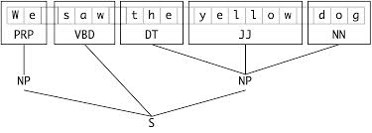
\includegraphics[width=0.8\linewidth,keepaspectratio]{postagging}
%%\end{center}
%%\end{frame}
%%
%%%%%%%%%%%%%%%%%%%%%%%%%%%%%%%%%%%%%%%%%%%%%%%%%%%%%%%%%%%%%%%%%%%%%%%%%%%%%%%%%%%%
%%\begin{frame}[fragile]\frametitle{NLTKs POS Tag Sets* - 1/2}
%%\begin{center}
%%
\includegraphics[width=0.8\linewidth,keepaspectratio]{postagging1}
%%\end{center}
%%\end{frame}
%%
%%
%%%%%%%%%%%%%%%%%%%%%%%%%%%%%%%%%%%%%%%%%%%%%%%%%%%%%%%%%%%%%%%%%%%%%%%%%%%%%%%%%%%%
%%\begin{frame}[fragile]\frametitle{NLTKs POS Tag Sets* - 2/2}
%%\begin{center}
%%
\includegraphics[width=0.8\linewidth,keepaspectratio]{postagging2}
%%\end{center}
%%\end{frame}
%%
%%%%%%%%%%%%%%%%%%%%%%%%%%%%%%%%%%%%%%%%%%%%%%%%%%%%%%%%%%%%%%%%%%%%%%%%%%%%%%%%%%%%
%%\begin{frame}[fragile]\frametitle{NLTK POS Tagger (Brown)}
%%\begin{lstlisting}
%%>>> nltk.pos_tag(brown.words()[:30])
%%[('The', 'DT'), ('Fulton', 'NNP'), ('County', 'NNP'), ('Grand', 'NNP'), ('Jury', 'NNP'), ('said', 'VBD'), ('Friday', 'NNP'), ('an', 'DT'), ('investigation', 'NN'), ('of', 'IN'), ("Atlanta's", 'JJ'), ('recent', 'JJ'), ('primary', 'JJ'), ('election', 'NN'), ('produced', 'VBN'), ('``', '``'), ('no', 'DT'), ('evidence', 'NN'), ("''", "''"), ('that', 'WDT'), ('any', 'DT'), ('irregularities', 'NNS'), ('took', 'VBD'), ('place', 'NN'), ('.', '.'), ('The', 'DT'), ('jury', 'NN'), ('further', 'RB'), ('said', 'VBD'), ('in', 'IN')]
%%>>> brown.tagged_words(simplify_tags=True)
%%[('The', 'DET'), ('Fulton', 'NP'), ('County', 'N'), ...]
%%\end{lstlisting}
%%\end{frame}
%%
%%%%%%%%%%%%%%%%%%%%%%%%%%%%%%%%%%%%%%%%%%%%%%%%%%%%%%%%%%%%%%%%%%%%%%%%%%%%%%%%%%%%
%%\begin{frame}[fragile]\frametitle{NLTK POS Dictionary}
%%\begin{lstlisting}
%%>>> pos = nltk.defaultdict(lambda:'N')
%%>>> pos['eat']
%%'N'
%%>>> pos.items()
%%[('eat', 'N')]
%%>>> for (word, tag) in brown.tagged_words(simplify_tags=True):
%%...     if word in pos:
%%...             if isinstance(pos[word], str):
%%...                     new_list = [pos[word]]
%%...                     pos[word] = new_list
%%...             if tag not in pos[word]:
%%...                     pos[word].append(tag)
%%...     else:
%%...             pos[word] = [tag]
%%... 
%%>>> pos['eat']
%%['N', 'V']
%%\end{lstlisting}
%%\end{frame}
%%
%%
%%
%%
%%
%%
%%
%%
%%
%%%%%%%%%%%%%%%%%%%%%%%%%%%%%%%%%%%%%%%%%%%%%%%%%%%%%%%%%%%%%%%%%%%%%%%%%%%%%%%%%%%%
%%\begin{frame}[fragile]\frametitle{Adding New Fields}
%%\small
%%
%%\begin{itemize}
%%\item Example: add CV field
%%\item Aside: utility function to do CV template
%%\end{itemize}
%%
%%\begin{lstlisting}
%%>>> import re
%%>>> def cv(s):
%%...     s = s.lower()
%%...     s = re.sub(r'[^a-z]',     r'_', s)
%%...     s = re.sub(r'[aeiou]',    r'V', s)
%%...     s = re.sub(r'[^V_]',      r'C', s)
%%...     return (s)
%%\end{lstlisting}
%%\end{frame}
%%
%%%%%%%%%%%%%%%%%%%%%%%%%%%%%%%%%%%%%%%%%%%%%%%%%%%%%%%%%%%%%%%%%%%%%%%%%%%%%%%%%%%%
%%\begin{frame}[fragile]\frametitle{Adding New Fields (cont)}
%%\small
%%
%%\begin{lstlisting}
%%>>> from nltk.etree.ElementTree import SubElement
%%>>> for entry in lexicon:
%%...     for field in entry:
%%...	    if field.tag == 'lx':
%%...         cv_field = SubElement(entry, 'cv')
%%...         cv_field.text = cv(field.text)
%%\end{lstlisting}
%%\end{frame}
%%
%%%%%%%%%%%%%%%%%%%%%%%%%%%%%%%%%%%%%%%%%%%%%%%%%%%%%%%%%%%%%%%%%%%%%%%%%%%%%%%%%%%%
%%\begin{frame}[fragile]\frametitle{Adding New Fields (cont)}
%%\scriptsize
%%\begin{lstlisting}
%%>>> toolbox.to_sfm_string(lexicon[50])
%%\lx kaeviro
%%\cv CVVCVCV
%%\ps V.A
%%\ge lift off
%%\ge take off
%%\gp go antap
%%\nt used to describe action of plane
%%\dt 12/Feb/2005
%%\ex Pita kaeviroroe kepa kekesia oa vuripierevo kiuvu.
%%\xp Pita i go antap na lukim haus win i bagarapim.
%%\xe Peter went to look at the house that the wind destroyed.
%%\end{lstlisting}
%%\end{frame}
%%
%%%%%%%%%%%%%%%%%%%%%%%%%%%%%%%%%%%%%%%%%%%%%%%%%%%%%%%%%%%%%%%%%%%%%%%%%%%%%%%%%%%%
%%\begin{frame}[fragile]\frametitle{Generating HTML Tables from Toolbox Data}
%%
%%\scriptsize
%%\begin{lstlisting}
%%>>> html = "<table>\n"
%%>>> for entry in lexicon[70:80]:
%%...     lx = entry.findtext('lx')
%%...     ps = entry.findtext('ps')
%%...     ge = entry.findtext('ge')
%%...     html += "  <tr><td>%s</td><td>%s</td><td>%s</td></tr>\n" %
%%...       (lx, ps, ge)
%%>>> html += "</table>"
%%>>> print html
%%\end{lstlisting}
%%
%%\tiny
%%
%%\begin{lstlisting}
%%<table>
%%  <tr><td>kakapikoto</td><td>N.N2</td><td>newborn baby</td></tr>
%%  <tr><td>kakapu</td><td>V.B</td><td>place in sling for purpose of carrying</td></tr>
%%  <tr><td>kakapua</td><td>N.N</td><td>sling for lifting</td></tr>
%%  <tr><td>kakara</td><td>N.N</td><td>bracelet</td></tr>
%%  <tr><td>Kakarapaia</td><td>N.PN</td><td>village name</td></tr>
%%  <tr><td>kakarau</td><td>N.F</td><td>stingray</td></tr>
%%  <tr><td>Kakarera</td><td>N.PN</td><td>name</td></tr>
%%  <tr><td>Kakareraia</td><td>N.???</td><td>name</td></tr>
%%  <tr><td>kakata</td><td>N.F</td><td>cockatoo</td></tr>
%%  <tr><td>kakate</td><td>N.F</td><td>bamboo tube for water</td></tr>
%%</table>
%%\end{lstlisting}
%%\end{frame}
%%
%%%%%%%%%%%%%%%%%%%%%%%%%%%%%%%%%%%%%%%%%%%%%%%%%%%%%%%%%%%%%%%%%%%%%%%%%%%%%%%%%%%%
%%\begin{frame}[fragile]\frametitle{Generating XML}
%%
%%\small
%%\begin{lstlisting}
%%>>> import sys
%%>>> from nltk.etree.ElementTree import ElementTree
%%>>> tree = ElementTree(lexicon[3])
%%>>> tree.write(sys.stdout)
%%\end{lstlisting}
%%
%%\scriptsize
%%\begin{lstlisting}
%%<record>
%%  <lx>kaakaaro</lx>
%%  <ps>N.N</ps>
%%  <ge>mixtures</ge>
%%  <gp>???</gp>
%%  <eng>mixtures</eng>
%%  <eng>charm used to keep married men and women youthful and attractive</eng>
%%  <cmt>Check vowel length. Is it kaakaaro or kaakaro?</cmt>
%%  <dt>14/May/2005</dt>
%%  <ex>Kaakaroto ira purapaiveira aue iava opita, voeao-pa airepa oraouirara, ra va aiopaive.</ex>
%%  <xp>Kokonas ol i save wokim long ol kain samting bilong ol nupela marit, bai ol i ken kaikai.</xp>
%%  <xe>Mixtures are made from coconut, ???.</xe>
%%</record>
%%\end{lstlisting}
%%\end{frame}
%%
%%%%%%%%%%%%%%%%%%%%%%%%%%%%%%%%%%%%%%%%%%%%%%%%%%%%%%%%%%%%%%%%%%%%%%%%%%%%%%%%%%%%
%%\begin{frame}[fragile]\frametitle{Analysis: Reduplication}
%%\scriptsize
%%\begin{itemize}
%%\item create a table of lexemes and their glosses
%%
%%\begin{lstlisting}
%%>>> lexgloss = {}
%%>>> for entry in lexicon:
%%...     lx = entry.findtext('lx')
%%...     if lx and entry.findtext('ps')[0] == 'V':
%%...         lexgloss[lx] = entry.findtext('ge')
%%\end{lstlisting}
%%
%%\item For each lexeme, check if the lexicon contains the reduplicated form:
%%
%%\begin{lstlisting}
%%>>> for lex in lexgloss:
%%...     if lex+lex in lexgloss:
%%...         print "%s (%s); %s (%s)" % (lex, lexgloss[lex], lex+lex, lexgloss[lex+lex])
%%\end{lstlisting}
%%\end{itemize}
%%\end{frame}
%%
%%%%%%%%%%%%%%%%%%%%%%%%%%%%%%%%%%%%%%%%%%%%%%%%%%%%%%%%%%%%%%%%%%%%%%%%%%%%%%%%%%%%
%%\begin{frame}[fragile]\frametitle{Reduplication (cont)}
%%\scriptsize
%%\begin{lstlisting}
%%kuvu (fill.up); kuvukuvu (stamp the ground)
%%kitu (save); kitukitu (scrub clothes)
%%kopa (ingest); kopakopa (gulp.down)
%%kasi (burn); kasikasi (angry)
%%koi (high pitched sound); koikoi (groan with pain)
%%kee (chip); keekee (shattered)
%%kauo (jump); kauokauo (jump up and down)
%%kea (deceived); keakea (lie)
%%kove (drop); kovekove (drip repeatedly)
%%kape (unable to meet); kapekape (grip with arms not meeting)
%%kapo (fasten.cover.strip); kapokapo (fasten.cover.strips)
%%koa (skin); koakoa (remove the skin)
%%kipu (paint); kipukipu (rub.on)
%%koe (spoon out a solid); koekoe (spoon out)
%%kovo (work); kovokovo (surround)
%%kiru (have sore near mouth); kirukiru (crisp)
%%kotu (bite); kotukotu (grind teeth together)
%%kavo (collect); kavokavo (work black magic)
%%...
%%\end{lstlisting}
%%\end{frame}
%%
%%%%%%%%%%%%%%%%%%%%%%%%%%%%%%%%%%%%%%%%%%%%%%%%%%%%%%%%%%%%%%%%%%%%%%%%%%%%%%%%%%%%
%%\begin{frame}[fragile]\frametitle{Complex Search Criteria}
%%\scriptsize
%%\begin{lstlisting}
%%>>> from nltk import tokenize, FreqDist
%%>>> fd = FreqDist()
%%>>> lexemes = [lexeme.text.lower() for lexeme in lexicon.findall('record/lx')]
%%>>> for lex in lexemes:
%%...     for syl in tokenize.regexp(lex, pattern=r'[^aeiou][aeiou]'):
%%...         fd.inc(syl)
%%\end{lstlisting}
%%
%%\normalsize
%%\begin{itemize}
%%\item for phonological description, identify segments, alternations,
%%  syllable canon...
%%\item what syllable types occur in lexemes (MSC, conspiracies)?
%%\end{itemize}
%%
%%\end{frame}
%%
%%%%%%%%%%%%%%%%%%%%%%%%%%%%%%%%%%%%%%%%%%%%%%%%%%%%%%%%%%%%%%%%%%%%%%%%%%%%%%%%%%%%
%%\begin{frame}[fragile]\frametitle{Analysis: Complex Search Criteria (cont)}
%%
%%\begin{itemize}
%%\item Tabulate the results:
%%
%%\scriptsize
%%\begin{lstlisting}
%%>>> for vowel in 'aeiou':
%%...     for cons in 'ptkvsr':
%%...          print '%s%s:%4d ' %
%%...            (cons, vowel, fd.count(cons+vowel)),
%%...     print
%%pa:  84  ta:  43  ka: 414  va:  87  sa:   0  ra: 185 
%%pe:  32  te:   8  ke: 139  ve:  25  se:   1  re:  62 
%%pi:  97  ti:   0  ki:  88  vi:  96  si:  95  ri:  83 
%%po:  31  to: 140  ko: 403  vo:  42  so:   3  ro:  86 
%%pu:  49  tu:  35  ku: 169  vu:  44  su:   1  ru:  72 
%%\end{lstlisting}
%%
%%\small
%%\item NB \texttt{t} and \texttt{s} columns
%%\item \texttt{ti} not attested, while \texttt{si} is frequent: palatalization?
%%\item which lexeme contains \texttt{su}?  \textit{kasuari}
%%\end{itemize}
%%\end{frame}
%%
%%%%%%%%%%%%%%%%%%%%%%%%%%%%%%%%%%%%%%%%%%%%%%%%%%%%%%%%%%%%%%%%%%%%%%%%%%%%%%%%%%%%
%%\begin{frame}[fragile]\frametitle{Analysis: Finding Minimal Sets}
%%\begin{itemize}
%%\item E.g. mace vs maze, face vs faze
%%\item minimal set parameters: context, target, display
%%\vfil
%%\small
%%
%%\begin{tabular}{l|lll}
%%\textbf{Minimal Set} &     \textbf{Context} &  \textbf{Target} & \textbf{Display} \\ \hline
%%\textit{bib, bid, big} &   first two letters&  third letter    & word\\
%%\textit{deal (N), deal (V)} & whole word    &  pos             & word (pos)
%%\end{tabular}
%%\end{itemize}
%%\end{frame}
%%
%%%%%%%%%%%%%%%%%%%%%%%%%%%%%%%%%%%%%%%%%%%%%%%%%%%%%%%%%%%%%%%%%%%%%%%%%%%%%%%%%%%%
%%\begin{frame}[fragile]\frametitle{Finding Minimal Sets: Example 1}
%%\scriptsize
%%
%%\begin{lstlisting}
%%>>> from nltk import MinimalSet
%%>>> pos = 1
%%>>> ms = MinimalSet((lex[:pos] + '_' + lex[pos+1:], lex[pos], lex)
%%...                 for lex in lexemes if len(lex) == 4)
%%>>> for context in ms.contexts(3):
%%...     print context + ':',
%%...     for target in ms.targets():
%%...         print "%-4s" % ms.display(context, target, "-"),
%%...     print
%%k_si: kasi -    kesi -    kosi
%%k_ru: karu kiru keru kuru koru
%%k_pu: kapu kipu -    -    kopu
%%k_ro: karo kiro -    -    koro
%%k_ri: kari kiri keri kuri kori
%%k_pa: kapa -    kepa -    kopa
%%k_ra: kara kira kera -    kora
%%k_ku: kaku -    -    kuku koku
%%k_ki: kaki kiki -    -    koki
%%\end{lstlisting}
%%\end{frame}
%%
%%%%%%%%%%%%%%%%%%%%%%%%%%%%%%%%%%%%%%%%%%%%%%%%%%%%%%%%%%%%%%%%%%%%%%%%%%%%%%%%%%%%
%%\begin{frame}[fragile]\frametitle{Finding Minimal Sets: Example 2}
%%\scriptsize
%%
%%\begin{lstlisting}
%%>>> entries = [(e.findtext('lx'), e.findtext('ps'), e.findtext('ge'))
%%...               for e in lexicon
%%...               if e.findtext('lx') and e.findtext('ps') and e.findtext('ge')]
%%>>> ms = MinimalSet((lx, ps[0], "%s (%s)" % (ps[0], ge))
%%...          for (lx, ps, ge) in entries)
%%>>> for context in ms.contexts()[:10]:
%%...     print "%10s:" % context, "; ".join(ms.display_all(context))
%%  kokovara: N (unripe coconut); V (unripe)
%%     kapua: N (sore); V (have sores)
%%      koie: N (pig); V (get pig to eat)
%%      kovo: C (garden); N (garden); V (work)
%%    kavori: N (crayfish); V (collect crayfish or lobster)
%%    korita: N (cutlet?); V (dissect meat)
%%      keru: N (bone); V (harden like bone)
%%  kirokiro: N (bush used for sorcery); V (write)
%%    kaapie: N (hook); V (snag)
%%       kou: C (heap); V (lay egg)
%%\end{lstlisting}
%%\end{frame}
%%
%%%%%%%%%%%%%%%%%%%%%%%%%%%%%%%%%%%%%%%%%%%%%%%%%%%%%%%%%%%%%%%%%%%%%%%%%%%%%%%%%%
\begin{frame}[fragile]\frametitle{}

\begin{center}
{\Large Language Resources}
\end{center}
\end{frame}

%%%%%%%%%%%%%%%%%%%%%%%%%%%%%%%%%%%%%%%%%%%%%%%%%%%%%%%%%%%%%%%%%%%%%%%%%%%%%%%%%%
\begin{frame}[fragile]\frametitle{ Accessing Data from NLTK }
\begin{itemize}
\item NLTK includes some corpora that are nothing more than wordlists (eg the Words Corpus)
\item What can they be useful for?
\item There is also a corpus of stopwords, that is, high-frequency words like the, to and also that we sometimes want to filter out of a document before further processing. 
\item Stopwords usually have little lexical content, and their presence in a text fails to distinguish it from other texts.
\begin{center}
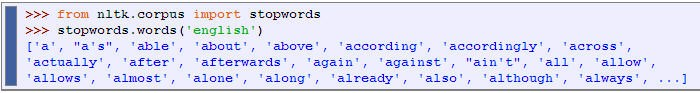
\includegraphics[width=\linewidth,keepaspectratio]{corp3}
\end{center}
\end{itemize}
\end{frame}

%%%%%%%%%%%%%%%%%%%%%%%%%%%%%%%%%%%%%%%%%%%%%%%%%%%%%%%%%%%%%%%%%%%%%%%%%%%%%%%%%%
\begin{frame}[fragile]\frametitle{Texts from Project Gutenberg}

{\small
\begin{lstlisting}
  >>> nltk.corpus.gutenberg.fileids()
  ['austen-emma', 'austen-persuasion', 'austen-sense', 'bible-kjv', 'blake-poems', 'blake-songs', 'chesterton-ball', 'chesterton-brown', 'chesterton-thursday', 'milton-paradise', 'shakespeare-caesar', 'shakespeare-hamlet', 'shakespeare-macbeth', 'whitman-leaves']
  >>> count = 0
  >>> for word in nltk.corpus.gutenberg.words('whitman-leaves'):
  ...     count += 1
  >>> print count
  154873
\end{lstlisting}}

{\tiny (Ref: https://www.nltk.org/book/ch02.html)}
\end{frame}

%%%%%%%%%%%%%%%%%%%%%%%%%%%%%%%%%%%%%%%%%%%%%%%%%%%%%%%%%%%%%%%%%%%%%%%%%%%%%%%%%%
\begin{frame}[fragile]\frametitle{Brown Corpus}
\scriptsize

\begin{lstlisting}
  >>> nltk.corpus.brown.fileids()
  ['a', 'b', 'c', 'd', 'e', 'f', 'g', 'h', 'j', 'k', 'l', 'm', 'n', 'p', 'r']
  >>> print nltk.corpus.brown.words('a')
  ['The', 'Fulton', 'County', 'Grand', 'Jury', 'said', 'Friday', 'an', 'investigation', 'of', ''Atlanta's'', 'recent', 'primary', 'election', 'produced', '``', 'no', 'evidence', '''''', 'that', 'any', 'irregularities', 'took', 'place', '.']
  >>> print nltk.corpus.brown.tagged_sents('a')
  [('The', 'at'), ('Fulton', 'np-tl'), ('County', 'nn-tl'), ('Grand', 'jj-tl'), ('Jury', 'nn-tl'), ('said', 'vbd'), ('Friday', 'nr'), ('an', 'at'), ('investigation', 'nn'), ('of', 'in'), (''Atlanta's'', 'np$'), ('recent', 'jj'), ('primary', 'nn'), ('election', 'nn'), ('produced', 'vbd'), ('``', '``'), ('no', 'at'), ('evidence', 'nn'), ('''''', ''''''), ('that', 'cs'), ('any', 'dti'), ('irregularities', 'nns'), ('took', 'vbd'), ('place', 'nn'), ('.', '.')]
\end{lstlisting}
\end{frame}




% %%%%%%%%%%%%%%%%%%%%%%%%%%%%%%%%%%%%%%%%%%%%%%%%%%%%%%%%%%%%%%%%%%%%%%%%%%%%%%%%%%
% \begin{frame}[fragile]\frametitle{Example: Genesis Corpora}
% \begin{itemize}
% \item Load a nltk corpus genesis

% {\small
% \begin{lstlisting}
% from nltk.corpus import genesis
% type(genesis)
% #nltk.corpus.reader.plaintext.PlaintextCorpusReader
% \end{lstlisting}}

% \item Get word counts as a dict

% {\small
% \begin{lstlisting}
% import collections 
% collections.Counter(genesis.words())

% Counter({'puhkesivat': 1,
         % 'cash': 1,
         % 'Kenen': 2,
         % 'resin': 1,
% ...})
% \end{lstlisting}}
% \end{itemize}
% \end{frame}

% %%%%%%%%%%%%%%%%%%%%%%%%%%%%%%%%%%%%%%%%%%%%%%%%%%%%%%%%%%%%%%%%%%%%%%%%%%%%%%%%%%
% \begin{frame}[fragile]\frametitle{Example: Genesis Corpora}
% \begin{itemize}
% \item Counter is same as following code

% {\small
% \begin{lstlisting}
% word_dict = {}
% for word in genesis.words():
    % if word in word_dict:
        % word_dict[word]+=1
    % else:
        % word_dict[word]=1

% print(word_dict)
% {'voimakkaat': 2,
 % 'cash': 1,
 % 'Kenen': 2,
% :
% }
% \end{lstlisting}}
% \item Sort on word counts
% {\small
% \begin{lstlisting}
% word_counts_sorted = sorted(word_dict.items(), 
                            % key=operator.itemgetter(1),
                            % reverse=True)
% print(word_counts_sorted)
% \end{lstlisting}}
% \end{itemize}
% \end{frame}

%%%%%%%%%%%%%%%%%%%%%%%%%%%%%%%%%%%%%%%%%%%%%%%%%%%%%%%%%%%%%%%%%%%%%%%%%%%%%%%%%%
\begin{frame}[fragile]\frametitle{Example: Genesis Corpora}
Zipf's Law: ``given a large sample of words used, the frequency of any word is inversely proportional to its rank in the frequency table''

Frequency Distribution of words in text. Assume that you have word\_counts\_sorted FreqDist.

{\scriptsize
\begin{lstlisting}
import matplotlib.pyplot as plt
import numpy as np
sample = word_counts_sorted[:25]
labels, values = [ combo[0] for (combo) in sample],[ combo[1] for combo in sample]
indexes = np.arange(len(labels))
plt.bar(indexes, values, 1)
plt.xticks(indexes + width * 0.5, labels)
plt.show()
\end{lstlisting}}
\begin{center}
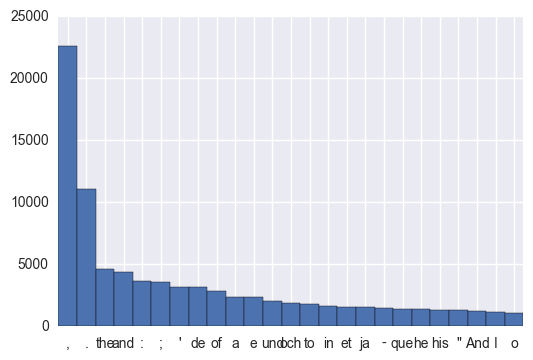
\includegraphics[width=0.3\linewidth,keepaspectratio]{genesisplot}
\end{center}
\end{frame}

%%%%%%%%%%%%%%%%%%%%%%%%%%%%%%%%%%%%%%%%%%%%%%%%%%%%%%%%%%%%%%%%%%%%%%%%%%%%%%%%%%
\begin{frame}[fragile]\frametitle{Exercise: Genesis Corpora}
{\small
\begin{lstlisting}
sample = word_counts_sorted[:100]
# Remove punctuation and plot the results
stripped_sample = [item[0].strip(",.!?;:") for item in sample]
labels_strip, values_strip = [ combo[0] for (combo) in stripped_list],[ combo[1] for combo in stripped_list]
indexes_strip = np.arange(len(labels_strip))
plt.figure(figsize=([20,5]))
plt.bar(indexes_strip, values_strip, 1)
plt.xticks(indexes_strip + width * .5, labels_strip)
plt.show()
\end{lstlisting}}
\begin{center}
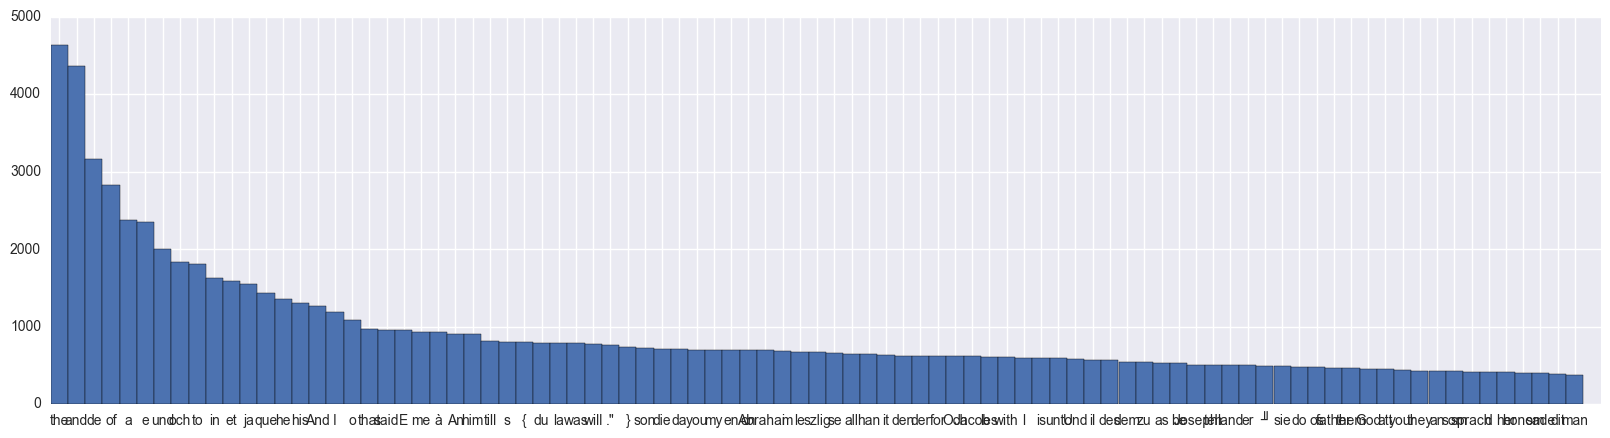
\includegraphics[width=0.32\linewidth,keepaspectratio]{genesisplot2}
\end{center}
\end{frame}

%%%%%%%%%%%%%%%%%%%%%%%%%%%%%%%%%%%%%%%%%%%%%%%%%%%%%%%%%%%%%%%%%%%%%%%%%%%%%%%%%
% \begin{frame}[fragile]\frametitle{Exercise: Genesis Corpora}
% {\small
% \begin{lstlisting}
% import pandas as pd

% pd.DataFrame(stripped_list).plot()
% #Only the first 100 words. More of a linear relationship
% plt.loglog([item[1] for item in stripped_list])
% #All the words in the corpus
% plt.loglog([item[1] for item in word_counts_sorted ])
% \end{lstlisting}}
% \begin{center}
% 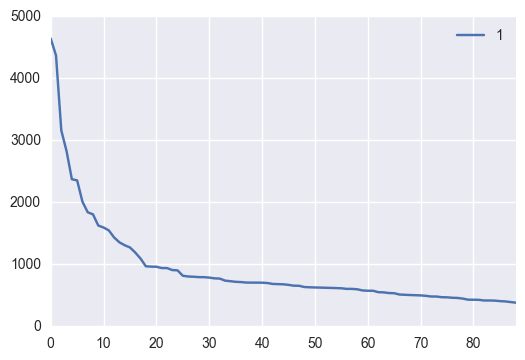
\includegraphics[width=0.32\linewidth,keepaspectratio]{genesisplot3}
% 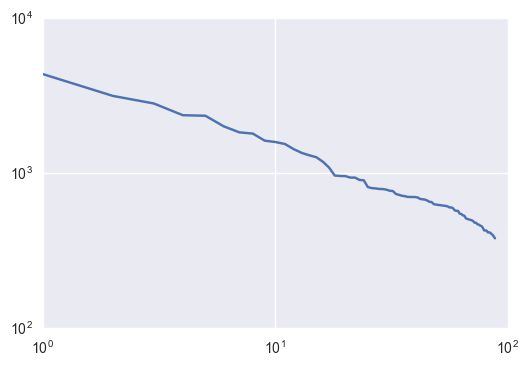
\includegraphics[width=0.32\linewidth,keepaspectratio]{genesisplot4}
% 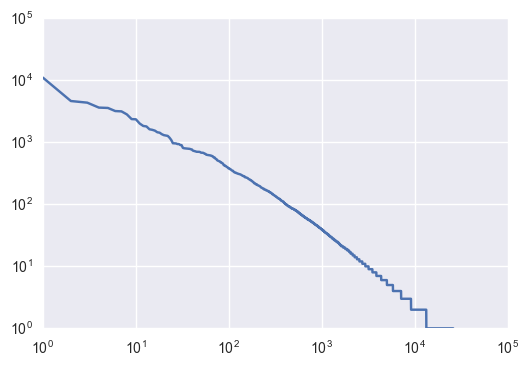
\includegraphics[width=0.32\linewidth,keepaspectratio]{genesisplot5}
% \end{center}
% \end{frame}


% %%%%%%%%%%%%%%%%%%%%%%%%%%%%%%%%%%%%%%%%%%%%%%%%%%%%%%%%%%%%%%%%%%%%%%%%%%%%%%%%%%%
% \begin{frame}[fragile]
% \frametitle{Accessing Data from the web}
% \begin{center}
% 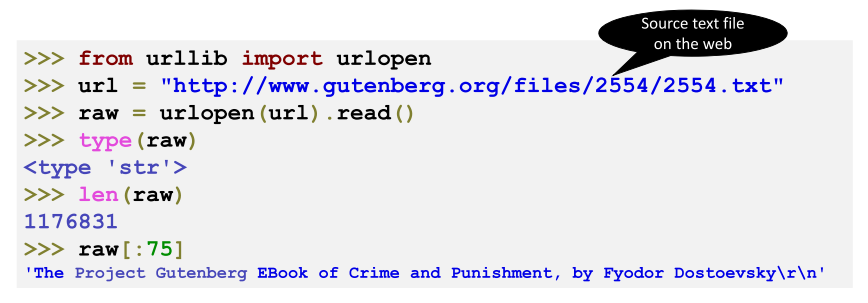
\includegraphics[width=\linewidth,keepaspectratio]{dataweb1}
% \end{center}
% \end{frame}

%%%%%%%%%%%%%%%%%%%%%%%%%%%%%%%%%%%%%%%%%%%%%%%%%%%%%%%%%%%%%%%%%%%%%%%%%%%%%%%%%%
\begin{frame}[fragile]\frametitle{Accessing Web Text}


\begin{lstlisting}
>>> import urllib, nltk
>>> html = urllib.urlopen('http://en.wikipedia.org/').read()
>>> text = nltk.clean_html(html)
>>> text.split()
['Wikimedia', 'Error', 'WIKIMEDIA', 'FOUNDATION', 'Fout', 'Fel',
'Fallo', '\xe9\x94\x99\xe8\xaf\xaf', '\xe9\x8c\xaf\xe8\xaa\xa4',
'Erreur', 'Error', 'Fehler', '\xe3\x82\xa8\xe3\x83\xa9\xe3\x83\xbc',
'B\xc5\x82\xc4\x85d', 'Errore', 'Erro', 'Chyba', 'EnglishThe',
'Wikimedia', 'Foundation', 'servers', 'are', 'currently',
'experiencing', 'technical', 'difficulties.The', 'problem', 'is',
'most', 'likely', 'temporary', 'and', 'will', 'hopefully', 'be',
'fixed', 'soon.', 'Please', 'check', 'back', 'in', 'a', 'few',
'minutes.For', 'further', 'information,', 'you', 'can', 'visit',
'the', 'wikipedia', 'channel', 'on', 'the', 'Freenode', 'IRC', ...
\end{lstlisting}
\end{frame}



% %%%%%%%%%%%%%%%%%%%%%%%%%%%%%%%%%%%%%%%%%%%%%%%%%%%%%%%%%%%%%%%%%%%%%%%%%%%%%%%%%%%
% \begin{frame}[fragile]
% \frametitle{Dealing with HTML}
% \begin{center}
% 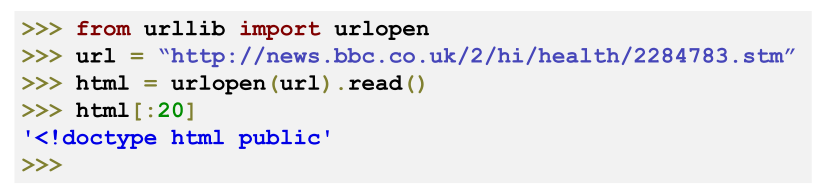
\includegraphics[width=\linewidth,keepaspectratio]{html1}
% \end{center}
% Need to get rid off the HTML markups.
% \end{frame}

% %%%%%%%%%%%%%%%%%%%%%%%%%%%%%%%%%%%%%%%%%%%%%%%%%%%%%%%%%%%%%%%%%%%%%%%%%%%%%%%%%%%
% \begin{frame}[fragile]
% \frametitle{Beautiful Soup Example}
% \begin{center}
% 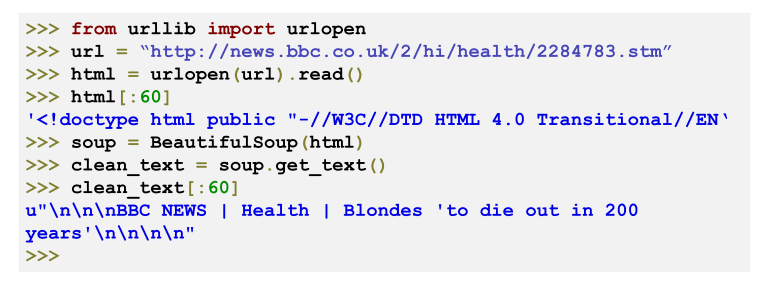
\includegraphics[width=\linewidth,keepaspectratio]{html2}
% \end{center}

% \end{frame}

%
%%%%%%%%%%%%%%%%%%%%%%%%%%%%%%%%%%%%%%%%%%%%%%%%%%%%%%%%%%%%%%%%%%%%%%%%%%%%%%%%%%%%
%\begin{frame}[fragile]
%\frametitle{String Operations (Review)}
%Accessing individual characters and sub-strings using slicing
%\begin{center}
%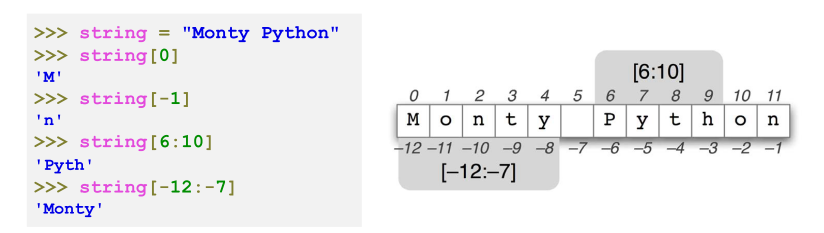
\includegraphics[width=\linewidth,keepaspectratio]{string1}
%\end{center}
%
%\end{frame}
%
%%%%%%%%%%%%%%%%%%%%%%%%%%%%%%%%%%%%%%%%%%%%%%%%%%%%%%%%%%%%%%%%%%%%%%%%%%%%%%%%%%%%
%\begin{frame}[fragile]
%\frametitle{String Operations (Review)}
%\begin{center}
%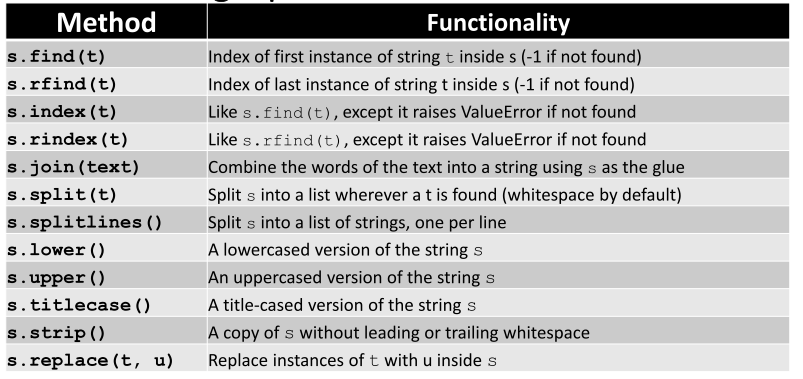
\includegraphics[width=\linewidth,keepaspectratio]{string2}
%\end{center}
%
%\end{frame}

%%%%%%%%%%%%%%%%%%%%%%%%%%%%%%%%%%%%%%%%%%%%%%%%%%%%%%%%%%%%%%%%%%%%%%%%%%%%%%%%%%
\begin{frame}[fragile]\frametitle{Accessing Spreadsheets}
File:
\begin{lstlisting}
dict.csv:
''sleep'',''sli:p'',''v.i'',''a condition of body and mind ...''
''walk'',''wo:k'',''v.intr'',''progress by lifting and setting down each foot ...''
''wake'',''weik'',''intrans'',''cease to sleep''

\end{lstlisting}

Import:

\begin{lstlisting}
>>> import csv
>>> file = open(''dict.csv'', ''rb'')
>>> for row in csv.reader(file):
...     print row
['sleep', 'sli:p', 'v.i', 'a condition of body and mind ...']
['walk', 'wo:k', 'v.intr', 'progress by lifting and setting down each foot ...']
['wake', 'weik', 'intrans', 'cease to sleep']
\end{lstlisting}
\end{frame}
%
%%%%%%%%%%%%%%%%%%%%%%%%%%%%%%%%%%%%%%%%%%%%%%%%%%%%%%%%%%%%%%%%%%%%%%%%%%%%%%%%%%%
%\begin{frame}[fragile]\frametitle{Data Cleansing: Validation}
%\small
%\begin{lstlisting}
%    def undefined_words(csv_file):
%        import csv
%        lexemes = set()
%        defn_words = set()
%        for row in csv.reader(open(csv_file)):
%            lexeme, pron, pos, defn = row
%            lexemes.add(lexeme)
%            defn_words.union(defn.split())
%        return sorted(defn_words.difference(lexemes))
%        
%    >>> print undefined_words(''dict.csv'')
%    ['...', 'a', 'and', 'body', 'by', 'cease',
%     'condition', 'down', 'each', 'foot',
%     'lifting', 'mind', 'of', 'progress',
%     'setting', 'to']
%\end{lstlisting}
%\end{frame}



%%%%%%%%%%%%%%%%%%%%%%%%%%%%%%%%%%%%%%%%%%%%%%%%%%%%%%%%%%%%%%%%%%%%%%%%%%%%%%%%%%%
%\begin{frame}[fragile]\frametitle{Accessing Toolbox Data}
%
%\begin{itemize}
%\item scan the file, convert into tree object
%\item preserves order of fields, gives array and XPath-style access
%\end{itemize}
%
%\scriptsize
%\begin{lstlisting}
%>>> from nltk.corpus import toolbox
%>>> lexicon = toolbox.xml('rotokas.dic')
%\end{lstlisting}
%\end{frame}
%
%%%%%%%%%%%%%%%%%%%%%%%%%%%%%%%%%%%%%%%%%%%%%%%%%%%%%%%%%%%%%%%%%%%%%%%%%%%%%%%%%%%
%\begin{frame}[fragile]\frametitle{Accessing with Indexes}
%
%\begin{lstlisting}
%>>> lexicon[3][0] 
%<Element lx at 77bd28>
%>>> lexicon[3][0].tag
%'lx'
%>>> lexicon[3][0].text
%'kaa'
%\end{lstlisting}
%\end{frame}
%
%%%%%%%%%%%%%%%%%%%%%%%%%%%%%%%%%%%%%%%%%%%%%%%%%%%%%%%%%%%%%%%%%%%%%%%%%%%%%%%%%%%
%\begin{frame}[fragile]\frametitle{Accessing with Indexes (cont)}
%
%\scriptsize
%\begin{lstlisting}
%>>> print nltk.corpus.reader.toolbox.to_sfm_string(lexicon[3])
%\lx kaa
%\ps N.M
%\cl isi
%\ge cooking banana
%\gp banana bilong kukim
%\sf FLORA
%\dt 12/Feb/2005
%\ex Taeavi iria kaa isi kovopaueva kaparapasia.
%\xp Taeavi i bin planim gaden banana bilong kukim tasol long paia.
%\xe Taeavi planted banana in order to cook it.
%\end{lstlisting}
%\end{frame}
%
%%%%%%%%%%%%%%%%%%%%%%%%%%%%%%%%%%%%%%%%%%%%%%%%%%%%%%%%%%%%%%%%%%%%%%%%%%%%%%%%%%%
%\begin{frame}[fragile]\frametitle{Accessing with Paths}
%
%\scriptsize
%\begin{lstlisting}
%>>> [lexeme.text.lower() for lexeme in lexicon.findall('record/lx')]
%['kaa', 'kaa', 'kaa', 'kaakaaro', 'kaakaaviko', 'kaakaavo', 'kaakaoko',
%'kaakasi', 'kaakau', 'kaakauko', 'kaakito', 'kaakuupato', ..., 'kuvuto']
%\end{lstlisting}
%
%\small
%\begin{itemize}
%\item lexicon is a series of \texttt{record} objects
%\item each contains field objects, such as \texttt{lx} and \texttt{ps}
%\item address all the lexemes: \texttt{record/lx}
%\end{itemize}
%\end{frame}

% %%%%%%%%%%%%%%%%%%%%%%%%%%%%%%%%%%%%%%%%%%%%%%%%%%%%%%%%%%%%%%%%%%%%%%%%%%%%%%%%%%
% \begin{frame}[fragile]\frametitle{Top-Down Design}
% \begin{itemize}
% \item Break down high-level task into manageable components
% \item Build and test each component
% \item Assemble them into a complex system
% \item Example: identify adjective-noun collocations in text
 % \begin{itemize}
 % \item read in the corpus
 % \item count events (each adjective, noun, adj-noun combination)
 % \item compute $\chi^2$ statistics
 % \item sort adj-noun pairs in decreasing order
 % \item output $n$-most significant collocations
 % \end{itemize}
% \item what are the inputs and outputs of each step (i.e. \textit{interfaces})
% \end{itemize}
% \end{frame}

% %%%%%%%%%%%%%%%%%%%%%%%%%%%%%%%%%%%%%%%%%%%%%%%%%%%%%%%%%%%%%%%%%%%%%%%%%%%%%%%%%%
% \begin{frame}[fragile]\frametitle{Top-Down Design (cont)}

% \begin{itemize}
% \item Define top-level function:

% \begin{lstlisting}
% def colloc(corpus_name, num):
   % corpus = load_corpus(corpus_name)
   % a_counts, n_counts, a_n_counts = count(corpus, 'JJ', 'NN')
   % a_n_scores = chisq(a_counts, n_counts, a_n_counts)
   % a_n_ranked = sort_by_score(a_n_scores)
   % return a_n_ranked[:num]
% \end{lstlisting}

% \item Iteratively define lower-level functions, e.g. \texttt{chisq()}

% \item Bottom-up testing
% \begin{itemize}
% \item standard test cases for components, known output
% \item only assemble once each component is known to work correctly
 % on the test cases
% \end{itemize}
% \end{itemize}
% \end{frame}

% %%%%%%%%%%%%%%%%%%%%%%%%%%%%%%%%%%%%%%%%%%%%%%%%%%%%%%%%%%%%%%%%%%%%%%%%%%%%%%%%%%
% \begin{frame}[fragile]\frametitle{Debugging}

 % \begin{itemize}
 % \item What's in the name:
   % \begin{itemize}
   % \item problems are small relative to their impact
   % \item hard-to-find
   % \item seem to take on a life of their own as the programmer tries to
     % hunt them down
   % \end{itemize}
 % \item steps:
   % \begin{itemize}
   % \item isolate the problem
   % \item syntax error: see error messages, linked to line numbers
   % \item run-time error: \textit{stack-trace}
   % \item add diagnostic print statements
   % \item display values of variables just before problem
   % \item Python debugger: \texttt{pdb}
   % \end{itemize}
 % \end{itemize}
% \end{frame}


%%%%%%%%%%%%%%%%%%%%%%%%%%%%%%%%%%%%%%%%%%%%%%%%%%%%%%%%%%%%%%%%%%%%%%%%%%%%%%%%%%
\begin{frame}[fragile]\frametitle{Getting Involved}
 \begin{itemize}
 \item http://nltk.org/
   \begin{itemize}
   \item http://nltk.org/index.php/Development
   \item http://nltk.org/index.php/Chatroom
   \end{itemize}
 \item Mailing lists:
   \begin{itemize}
   \item nltk-devel@lists.sourceforge.net
   \item nltk-announce@lists.sourceforge.net
   \item nltk-users@lists.sourceforge.net
   \end{itemize}
 \end{itemize}
\end{frame}

